\documentclass[unknownkeysallowed]{beamer}
\usepackage[french,english]{babel}
\usepackage{./sty/beamer_js}
\usepackage{./sty/shortcuts_js}
\usepackage{csquotes}


\addbibresource{Bibliographie.bib}
\usepackage{enumerate}

\begin{document}


%%%%%%%%%%%%%%%%%%%%%%%%%%%%%%%%%%%%%%%%%%%%%%%%%%%%%%%%%%%%%%%%%%%%%%%%%%%%%%%
%%%%%%%%%%%%%%%%%%%%%%             Headers               %%%%%%%%%%%%%%%%%%%%%%
%%%%%%%%%%%%%%%%%%%%%%%%%%%%%%%%%%%%%%%%%%%%%%%%%%%%%%%%%%%%%%%%%%%%%%%%%%%%%%%



%%%%%%%%%%%%%%%%%%%%%%%%%%%%%%%%%%%%%%%%%%%%%%%%%%%%%%%%%%%%%%%%%%%%%%%%%%%%%%%
\begin{frame}[noframenumbering]
\thispagestyle{empty}
\bigskip
\bigskip
\begin{center}{
\LARGE\color{marron}
\textbf{HMMA 307 : Modèles linéaires avancés}
\textbf{ }\\
\vspace{0.5cm}
}

\color{marron}
\textbf{Robustesse des modèles linéaires à effets mixtes face aux violations des hypothèses de distribution}
\end{center}

\vspace{0.5cm}

\begin{center}
\textbf{ GAIZI IBRAHIM  } \\
\vspace{0.1cm}
\url{https://github.com/ibrahimgaizi1}\\
\vspace{0.5cm}
Université de Montpellier \\
\end{center}

\centering

\includegraphics[width=0.13\textwidth]{logo.png}
\end{frame}


%%%%%%%%%%%%%%%%%%%%%%%%%%%%%%%%%%%%%%%%%%%%%%%%%%%%%%%%%%%%%%%%%%%%%%%%%%%%%%%
%%%%%%%%%%%%%%%%%%%%%%%%%   table of contents     %%%%%%%%%%%%%%%%%%%%%%%%%%%%%
%%%%%%%%%%%%%%%%%%%%%%%%%%%%%%%%%%%%%%%%%%%%%%%%%%%%%%%%%%%%%%%%%%%%%%%%%%%%%%%

\begin{frame}[noframenumbering]
\thispagestyle{empty}
\tableofcontents
\end{frame}





%%%%%%%%%%%%%%%%%%%%%%%%%%%%%%%%%%%%%%%%%%%%%%%%%%%%%%%%%%%%%%%%%%%%%%%%%%%%%%%
%%%%%%%%%%%%%%%%%%%%%%          Presentation figure      %%%%%%%%%%%%%%%%%%%%%%
%%%%%%%%%%%%%%%%%%%%%%%%%%%%%%%%%%%%%%%%%%%%%%%%%%%%%%%%%%%%%%%%%%%%%%%%%%%%%%%

%%%%%%%%%%%%%%%%%%%%%%%%%%%%%%%%%%%%%%%%%%%%%%%%%%%%%%%%%%%%%%%%%%%%%%%%%%%%%%%
%%%%%%%%%%%%%%%%    Introduction   %%%%%%%%%%%%%%%%%%%%%%
%%%%%%%%%%%%%%%%%%%%%%%%%%%%%%%%%%%%%%%%%%%%%%%%%%%%%%%%%%%%%%%%%%%%%%%%%%%%%%%
\begin{frame}{{Introduction :} }

 \begin{itemize}
        \item Outils puissants pour analyser des ensembles de données complexes avec des observations répétées ou groupées.
        \item Impliquent des procédures d'ajustement sur la distribution des effets résiduels et aléatoires.
        \item les hypothèses de distribution des effets aléatoires ne peuvent pas être vérifiées aussi facilement que pour les effets fixes 
    \end{itemize}
\end{frame}

%%%%%%%%%%%%%%%%%%%%%%%%%%%%%%%%%%%%%%%%%%%%%%%%%%%%%%%%%%%%%%%%%%%%%%%%%%%%%%
%%%%%%%%%%%%%%%%%%%%%%%      modèle à effets linéaires mixtes     %%%%%%%%%%%%%%%%%%%%%%%%%%%%%%%%%%
%%%%%%%%%%%%%%%%%%%%%%%%%%%%%%%%%%%%%%%%%%%%%%%%%%%%%%%%%%%%%%%%%%%%%%%%%%%%%

\begin{frame}{Les modèles à effets linéaires mixtes}
\section{Simulation des données :}
\begin{alertblock}{Modèle de base simulé}


$$ y=\beta_0+\beta_1 x_1+\beta_2x_2+\hat{\alpha}+\hat{\epsilon}  $$
$$ \hat{\alpha} \sim  N(0,\hat{\sigma}^2_{\hat{\alpha}}) $$
$$ \hat{\epsilon} \sim  N(0,\hat{\sigma}^2_{\hat{\epsilon}}) $$

$\hat{\beta_0},\hat{\beta_1},\hat{\beta_2},\hat{\alpha},\hat{\epsilon}$     sont respectivement les approximations de :  $\beta_0,\beta_1,\beta_2,\alpha,\epsilon.$ 
\end{alertblock}

\medskip

 \begin{itemize}
        \item Simuler des données et à les ajuster dans un simple LMM
        \item Enfreindre les hypothèses sur les effets aléatoires et les distributions d'erreurs selon diffèrents scénarios .
   
    \end{itemize}
 
 


\end{frame}
%%%%%%%%%%%%%%%%%%%%%%%%%%%%%%%%%%%%%%%%%%%%%%%%%%%%%%%%%%%%%%%%%%%%%%%%%%%%%%
%%%%%%%%%%%%%%%%%%%%%%%     Comparaison entre OLS RLM    %%%%%%%%%%%%%%%%%%%%%%%%%%%%%%%%%%
%%%%%%%%%%%%%%%%%%%%%%%%%%%%%%%%%%%%%%%%%%%%%%%%%%%%%%%%%%%%%%%%%%%%%%%%%%%%%
  
  
  
  \begin{frame}{Comparaison entre OLS RLM : }

\begin{figure}
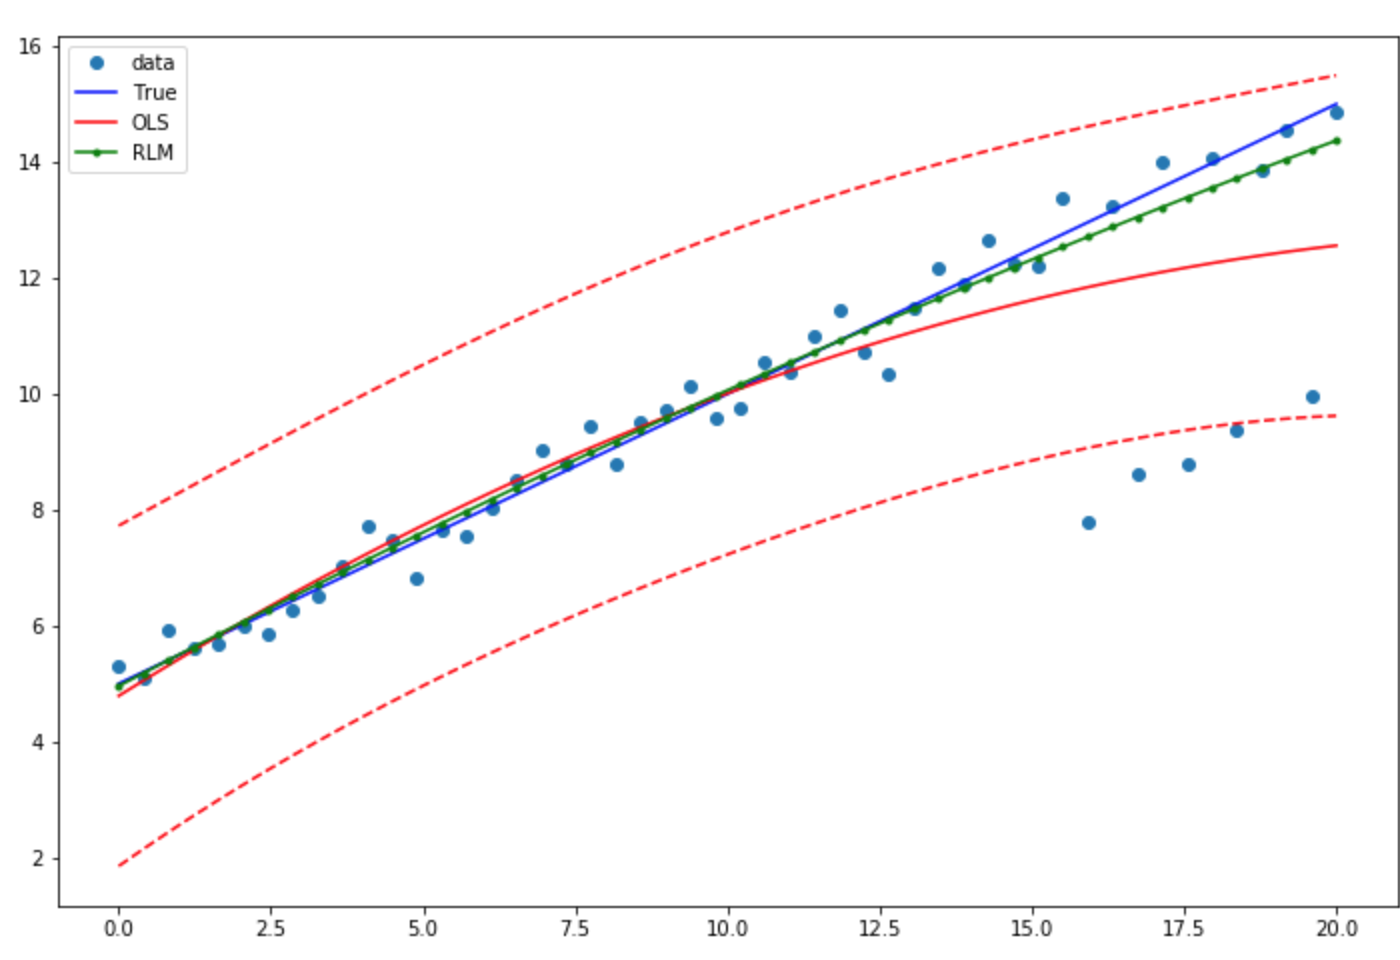
\includegraphics[scale=0.28]{0.png}
\caption{Comparaison entre les estimations avec les methodes RLM et OLS.}
\end{figure}
\end{frame}

  
  
  
  

%%%%%%%%%%%%%%%%%%%%%%%%%%%%%%%%%%%%%%%%%%%%%%%%%%%%%%%%%%%%%%%%%%%%%%%%%%%%%%%
%%%%%%%%%%%%%%%%%%%%%%      Scénarios A&B                  %%%%%%%%%%%%%%%%%%%%%%


\begin{frame}{Scénarios A et B}
\section{Les différents scénarios :}
 \textbf{\textit{Distributions biaisées (scénario A)}} :
 
 \begin{itemize}
 
        \item $\alpha$ et $\epsilon$ ont été tirés des distributions biaisées.

    \end{itemize}
 \textbf{\textit{Distributions bimodales (scénario B)}} :
 \begin{itemize}
 
        \item  Les distributions ont été tirées de deux distributions normales distinctes.
 				 \item  Les distributions ont des moyennes déplacées de  ±1,5 unités
  	 			\item La moitié des tirages est déplacée vers le bas et la moitié vers le haut.
  				\item La variance a été  réajustée
  \end{itemize}
\end{frame}


%%%%%%%%%%%%%%%%%%%%%%%%%%%%%%%%%%%%%%%%%%%%%%%%%%%%%%%%%%%%%%%%%%%%%%%%%%%%%%%


\begin{frame}{Scénarios C et D et E}
 \textbf{\textit{Distributions hétéroscédastiques (scénario C)}} :
 \begin{itemize}
 
        \item  $\alpha$ et $\epsilon$  sont tirées de distributions où la variance dépend d'une des covariables (x1)
    	\item  $\lambda$  prend les valeurs 2, 4 ou 8.
    \end{itemize}
 \textbf{\textit{Effets aléatoires manquants	 (scénario D)}} :
 \begin{itemize}
 
        \item  Effets  aléatoires échantillonnés de manière déséquilibrée,
  				\item  Variances à effet aléatoire fixées.
  \end{itemize}
   \textbf{\textit{Prédicteurs corrélés	 (scénarios E)}} :
 \begin{itemize}
 
        \item  Prédicteurs corrélés avec des corrélations fixées à +0,2, +0,5 et +0,8

  \end{itemize}
\end{frame}



\begin{frame}{Violation en biais}
\section{Violation des hypothèses de distribution :}
\begin{figure}
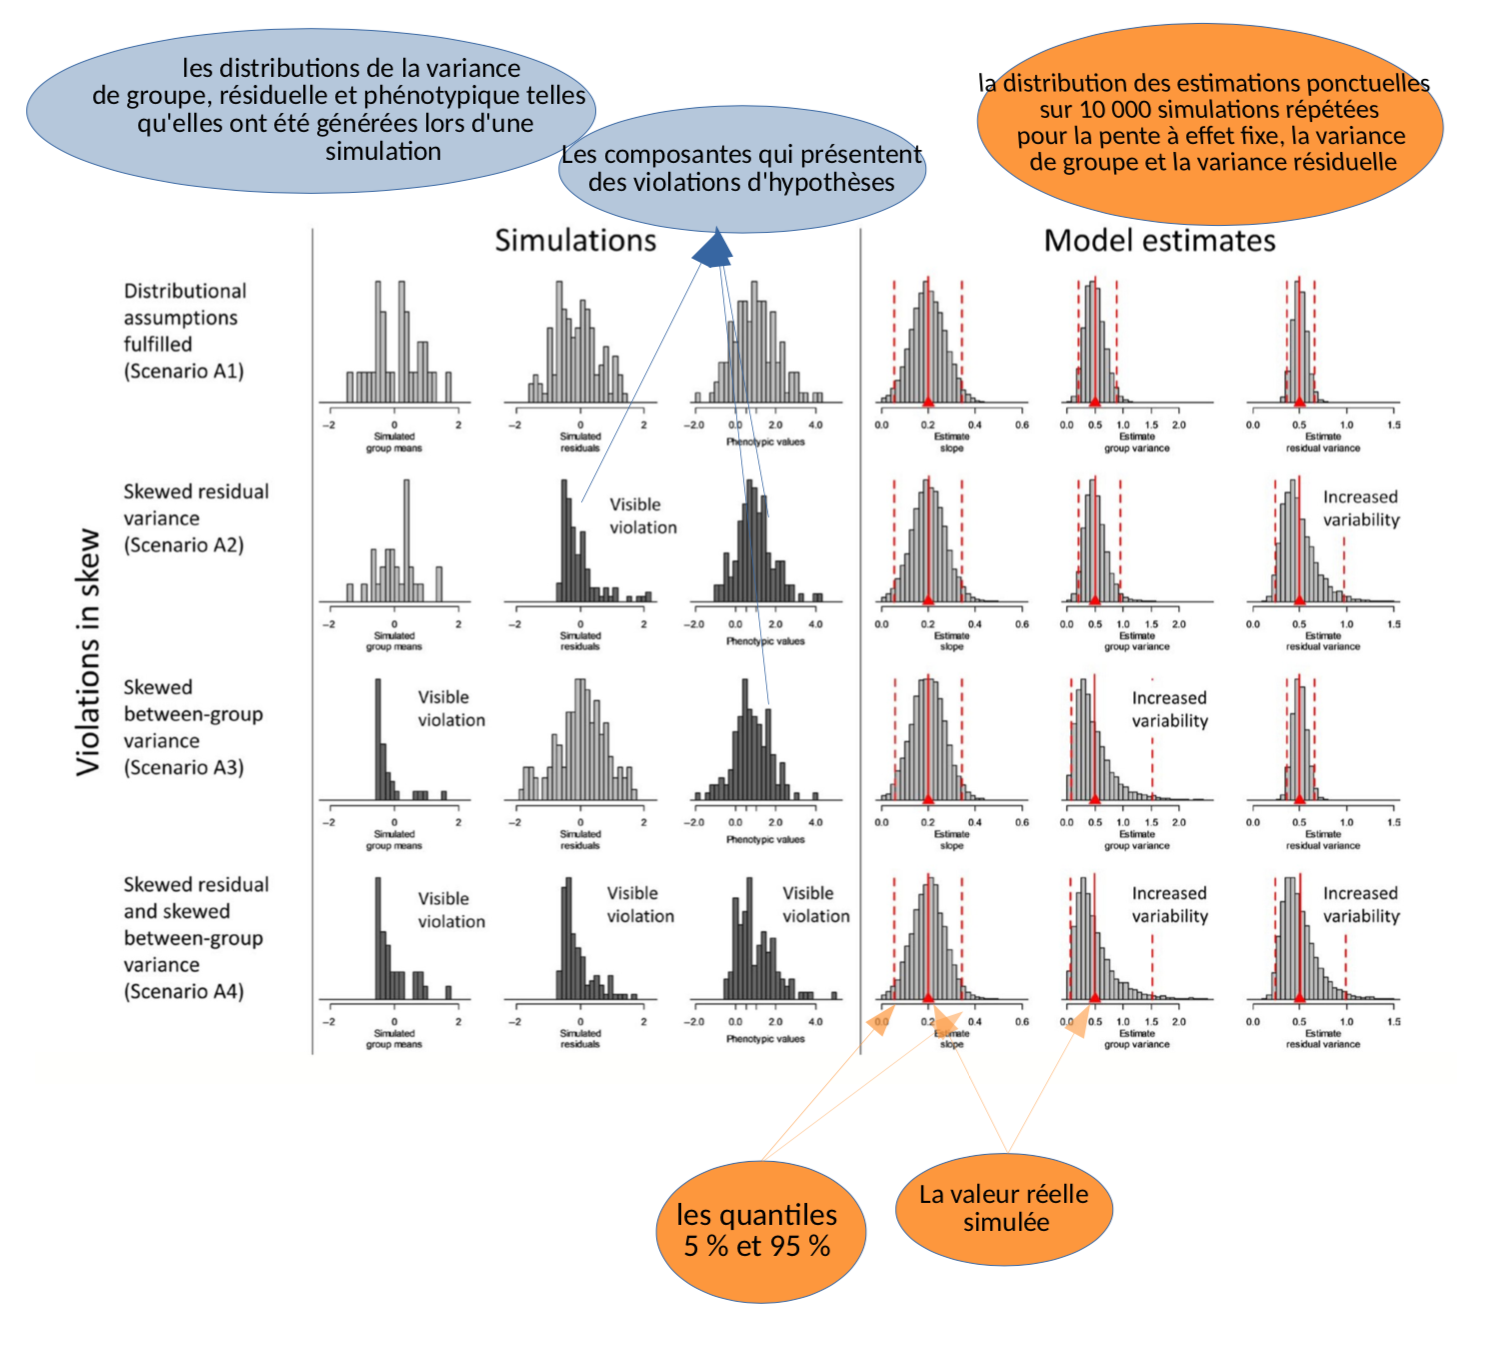
\includegraphics[scale=0.28]{11.png}
\caption{les effets des violations des hypothèses de distribution sur les estimations des paramètres d'intérêt majeur.}
\end{figure}
\end{frame}

\begin{frame}{Effets des distributions biaisées }

\begin{figure}
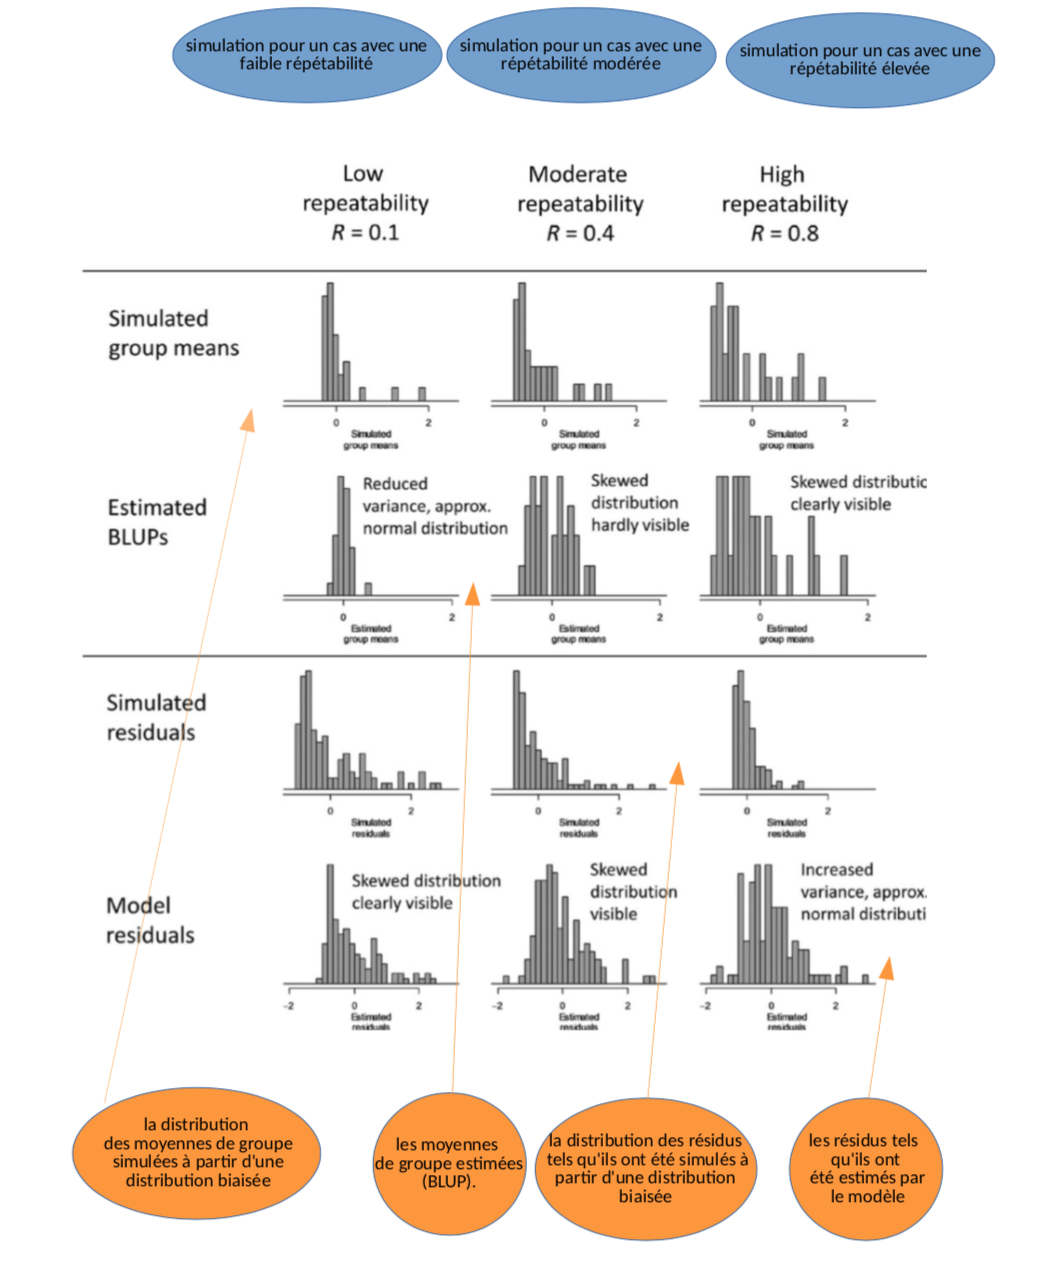
\includegraphics[scale=0.28]{2p.png}
\caption{Effets des distributions biaisées et de la taille des composantes de la variance sur les moyennes et les résidus estimés des groupes.}
\end{figure}
\end{frame}



\begin{frame}{Impactes des effets aléatoires manquants }

\begin{figure}
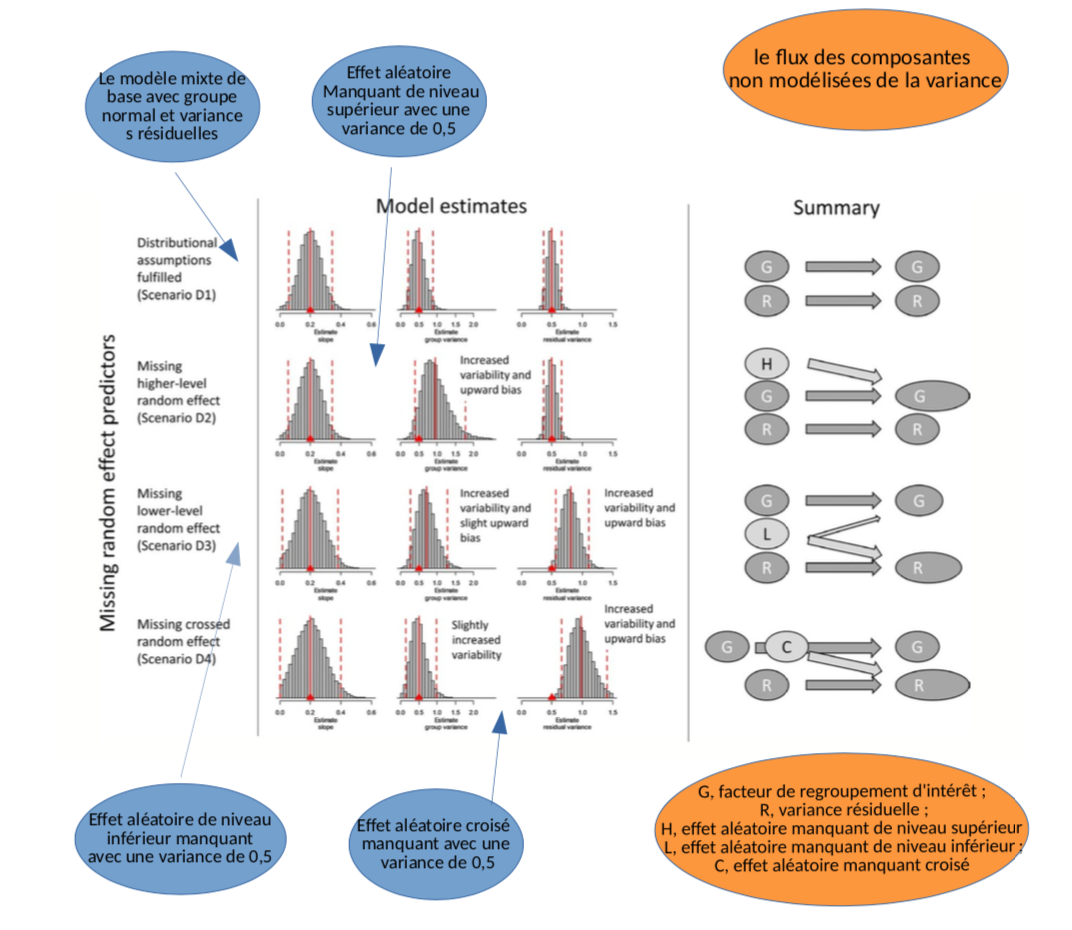
\includegraphics[scale=0.28]{4.png}
\caption{Effets des distributions biaisées et de la taille des composantes de la variance sur les moyennes et les résidus estimés des groupes.}
\end{figure}
\end{frame}


\begin{frame}{Biais et prédiction  }


\begin{figure}
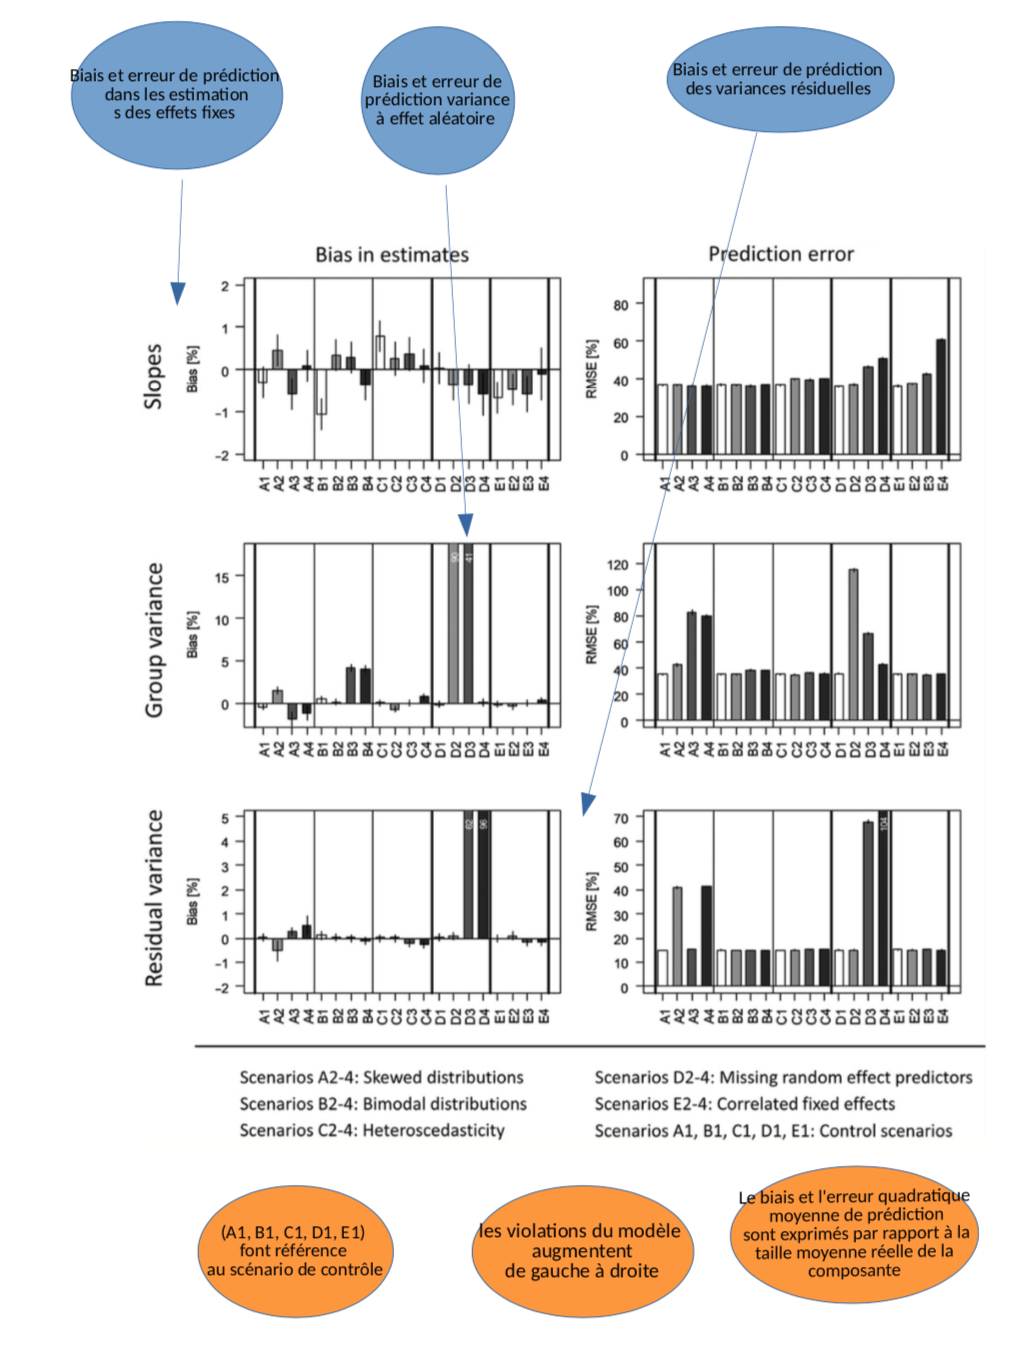
\includegraphics[scale=0.28]{5p.png}
\caption{Effets des distributions biaisées et de la taille des composantes de la variance sur les moyennes et les résidus estimés des groupes.}
\end{figure}
\end{frame}

\begin{frame}{Analyse : }
\section{Analyse des résultats :}
 \begin{itemize}
        \item L'effet des violations des hypothèses de distribution des variances à effet aléatoire et des résidus est  faible.
        \item Faible biais global sauf pour les distribution bimodale.
        \item Certaines violations simulées peuvent  émerger de modèles incomplets .			\item Les termes d'effet aléatoire manquants ont des effets systématiques sur les estimations d'autres composantes de la variance.
\item Il existe une imprécision accrue des estimations d'effets fixes lorsque les covariables sont corrélées.
\item Faible impact de l'hétéroscédasticité sur les estimations du modèle
    \end{itemize}

\end{frame}

\begin{frame}{Conclusion : }
 \begin{itemize}
        \item 
\Lesecs Modèles à effets mixtes sont largement robustes
        \item Ils ont un faible biais global sauf pour les distributions bimodales.
        \item Les violations hypothèses peuvent parfois entraîner une variabilité accrue des estimations.			
\item Outils puissants permettant de modéliser une grande variété d'ensembles de données. 
    \end{itemize}

\end{frame}





%%%%%%%%%%%%%%%%%%%%%%%%%%%%%%%%%%%%%%%%%%%%%%%%%%%%%%%%%%%%%%%%%%%%%%%%%%%%%
%%%%%%%%%%%%%%%%%%%%%%%%%%    Bibliography   %%%%%%%%%%%%%%%%%%%%%%%%%%%%%%%%
%%%%%%%%%%%%%%%%%%%%%%%%%%%%%%%%%%%%%%%%%%%%%%%%%%%%%%%%%%%%%%%%%%%%%%%%%%%%%

\begin{frame}{Bibliography}
\nocite{*}
\printbibliography
\end{frame}

\end{document}